\documentclass{beamer}
\mode<presentation>
\usetheme{Warsaw}
\usetheme[headheight=.4 in, footheight=.2in]{boxes}

\usepackage{etex}
\usepackage{graphicx, booktabs, tikz, color, subcaption, pgfplots}
\usepackage{pgf-umlsd}

\usepackage{enumerate}

\usepackage{ifthen}
\usetikzlibrary{shapes.misc, shapes, arrows}

\usetikzlibrary{matrix}
\usetikzlibrary{positioning}

% for animation
%\usepackage{xmpmulti}
\usepackage{animate}

%------------------------------------------
% Legend for tikzpicture

\newenvironment{customlegend}[1][]{
	\begingroup
	\csname pgfplots@init@cleared@structures
	\pgfplotsset{#1}
}{
	\csname pgfplots@createlegend
	\endgroup
}

\def\addlegendimage{\csname pgfplots@addlegendimage\endcsname}

%---------------------------------

\title{ Intro to GANs}
\author { Candice and Larry}
\vspace{.2cm}




\begin{document}

\begin{frame}[fragile]
	\titlepage
\end{frame}



\begin{frame}[fragile]

\begin{figure}
\begin{center}
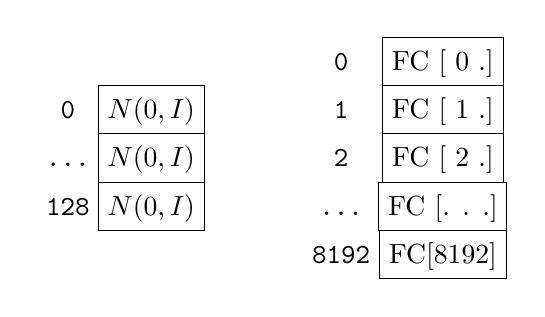
\begin{tikzpicture}[cell/.style={rectangle,draw=black},
space/.style={minimum height=1.5em,matrix of nodes,row sep=-\pgflinewidth,column sep=-\pgflinewidth,column 1/.style={font=\ttfamily}},text depth=0.5ex,text height=2ex,nodes in empty cells]
%[cell/.style={rectangle,draw=black},
%space/.style={minimum height=1.5em,matrix of nodes,row sep=-\pgflinewidth,column sep=-\pgflinewidth,column 1/.style={font=\ttfamily}}]

\matrix (first) [space, row sep=-\pgflinewidth, column 1/.style={font=\ttfamily},column 2/.style={nodes={cell,minimum width=2em}}]
{
0 & $N(0,I)$\\
... & $N(0,I)$ \\
128 & $N(0,I)$\\
};

\matrix (second) [right=of first, space, row sep=-\pgflinewidth, column 2/.style={minimum width=3em,nodes={cell,minimum width=3.5em}},column 3/.style={nodes={cell,minimum width=2em}}]
{
0   & FC   [  0       .] \\
1   &  FC   [  1      .] \\
2   & FC   [  2       .] \\
... & FC  [. . .]\\
8192 & FC[8192]\\
};

\end{tikzpicture}
\end{center}
\end{figure}

\begin{figure}
	\noindent\resizebox{\textwidth}{!}{

	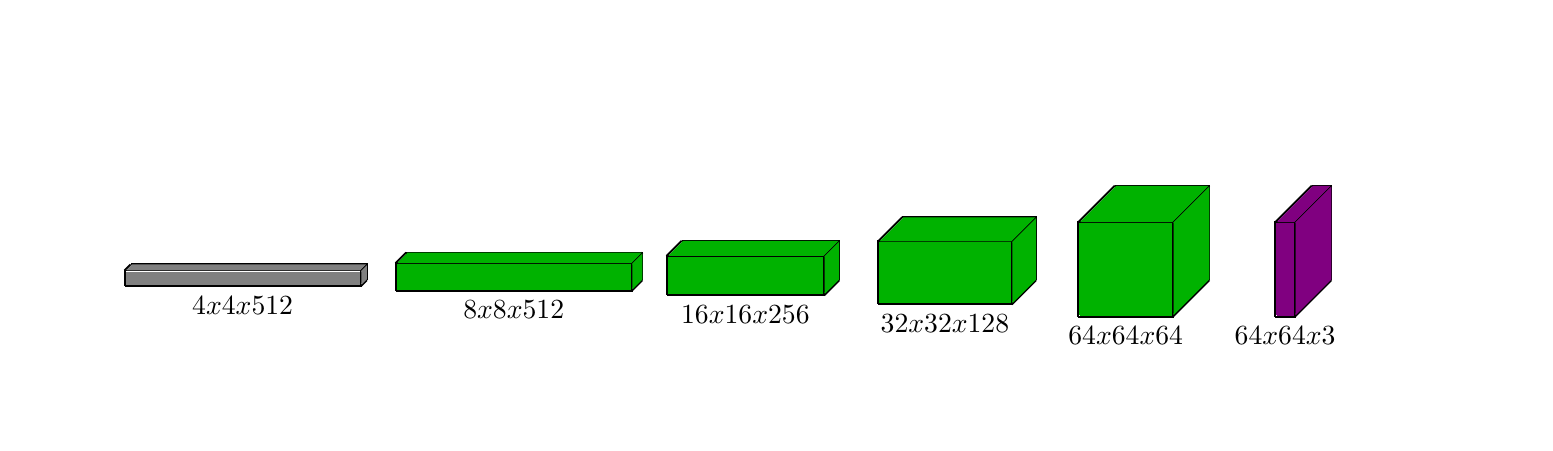
\begin{tikzpicture}
		\draw[use as bounding box, transparent] (-1.8,-1.8) rectangle (17.2, 3.2);

		% Define the macro.
		% 1st argument: Height and width of the layer rectangle slice.
		% 2nd argument: Depth of the layer slice
		% 3rd argument: X Offset --> use it to offset layers from previously drawn layers.
		% 4th argument: Options for filldraw.
		% 5th argument: Text to be placed below this layer.
		% 6th argument: Y Offset --> Use it when an output needs to be fed to multiple layers that are on the same X offset.

		\newcommand{\networkLayer}[6]{
			\def\a{#1} % Used to distinguish input resolution for current layer.
			\def\b{0.02}
			\def\c{#2} % Width of the cube to distinguish number of input channels for current layer.
			\def\t{#3} % X offset for current layer.
			\ifthenelse {\equal{#6} {}} {\def\y{0}} {\def\y{#6}} % Y offset for current layer.

			% Draw the layer body.
			\draw[line width=0.25mm](\c+\t,0,0) -- (\c+\t,\a,0) -- (\t,\a,0);                                                      % back plane
			\draw[line width=0.25mm](\t,0,\a) -- (\c+\t,0,\a) node[midway,below] {#5} -- (\c+\t,\a,\a) -- (\t,\a,\a) -- (\t,0,\a); % front plane
			\draw[line width=0.25mm](\c+\t,0,0) -- (\c+\t,0,\a);
			\draw[line width=0.25mm](\c+\t,\a,0) -- (\c+\t,\a,\a);
			\draw[line width=0.25mm](\t,\a,0) -- (\t,\a,\a);

			% Recolor visible surfaces
			\filldraw[#4] (\t+\b,\b,\a) -- (\c+\t-\b,\b,\a) -- (\c+\t-\b,\a-\b,\a) -- (\t+\b,\a-\b,\a) -- (\t+\b,\b,\a); % front plane
			\filldraw[#4] (\t+\b,\a,\a-\b) -- (\c+\t-\b,\a,\a-\b) -- (\c+\t-\b,\a,\b) -- (\t+\b,\a,\b);

			% Colored slice.
			\ifthenelse {\equal{#4} {}}
			{} % Do not draw colored slice if #4 is blank.
			{\filldraw[#4] (\c+\t,\b,\a-\b) -- (\c+\t,\b,\b) -- (\c+\t,\a-\b,\b) -- (\c+\t,\a-\b,\a-\b);} % Else, draw a colored slice.
		}

		% INPUT
		\networkLayer{0.2}{3.0}{-0.5}{color=gray}{$4x4x512$}{}

		% Generator
		\networkLayer{0.35}{3.0}{3.0}{color=black!30!green}{$8x8x512$}{}    % S1
		\draw [->];
		\networkLayer{0.5}{2.0}{6.5}{color=black!30!green}{$16x16x256$}{}        % S2
		\networkLayer{.8}{1.7}{9.3}{color=black!30!green}{$32x32x128$}{}    % S1
		\networkLayer{1.2}{1.2}{12.0}{color=black!30!green}{$64x64x64$}{}        % S2
		\networkLayer{1.2}{0.25}{14.5}{color=red!50!blue}{$64x64x3$}{}    % S1


	\end{tikzpicture}
	}
	\caption{Example Generator Architecture}
	\label{fig:cnn}

\end{figure}

Add footnote at bottom for gray = reshape, blue = upconv





\end{frame}


\begin{frame}
What really made this work was using [fragile] when starting the frame
\end{frame}


\begin{frame}{GAN framework}
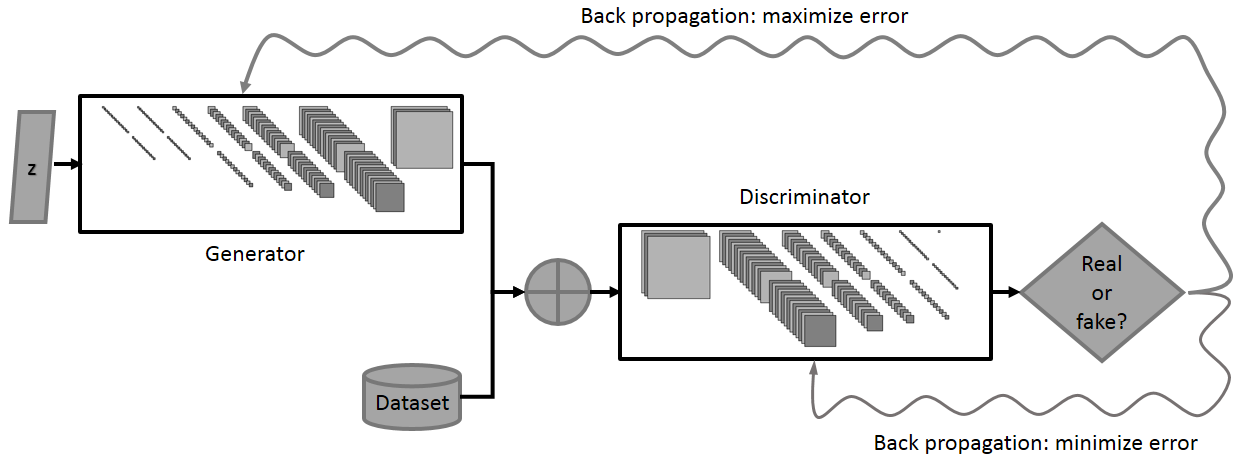
\includegraphics[scale=0.3]{gan_architecture_nvidia.png}
\end{frame}

\begin{frame}
Insert a gif here
%\transduration<0-16>{0}
%        \multiinclude[<+->][format=png, graphics={width=\textwidth}]{/home/crgerst/src/GAN/samples/CelebA/wgangp_test_CelebA_generator_size/something}
\animategraphics[height=2.8in,autoplay,loop]{1}{/home/crgerst/src/GAN/samples/CelebA/wgangp_test_CelebA_generator_size/something-}{0}{3}

\end{frame}


\begin{frame}
IC partner application
%\transduration<0-16>{0}
%        \multiinclude[<+->][format=png, graphics={width=\textwidth}]{/home/crgerst/src/GAN/samples/CelebA/wgangp_test_CelebA_generator_size/something}
\animategraphics[height=1in,autoplay,loop]{1}{fixed_person-}{0}{98}

\end{frame}

\end{document}
